\section{面向服务中的信息交换和数据类型}

\subsection{电子信息交换}
电子信息交换是指在执行领域(业务)相关功能时,各式各样、采用电子方式编码的信息,在软件单元之间的移动的过程。

\begin{figure}[H]
    \vspace{-0.5em}
	\centering
	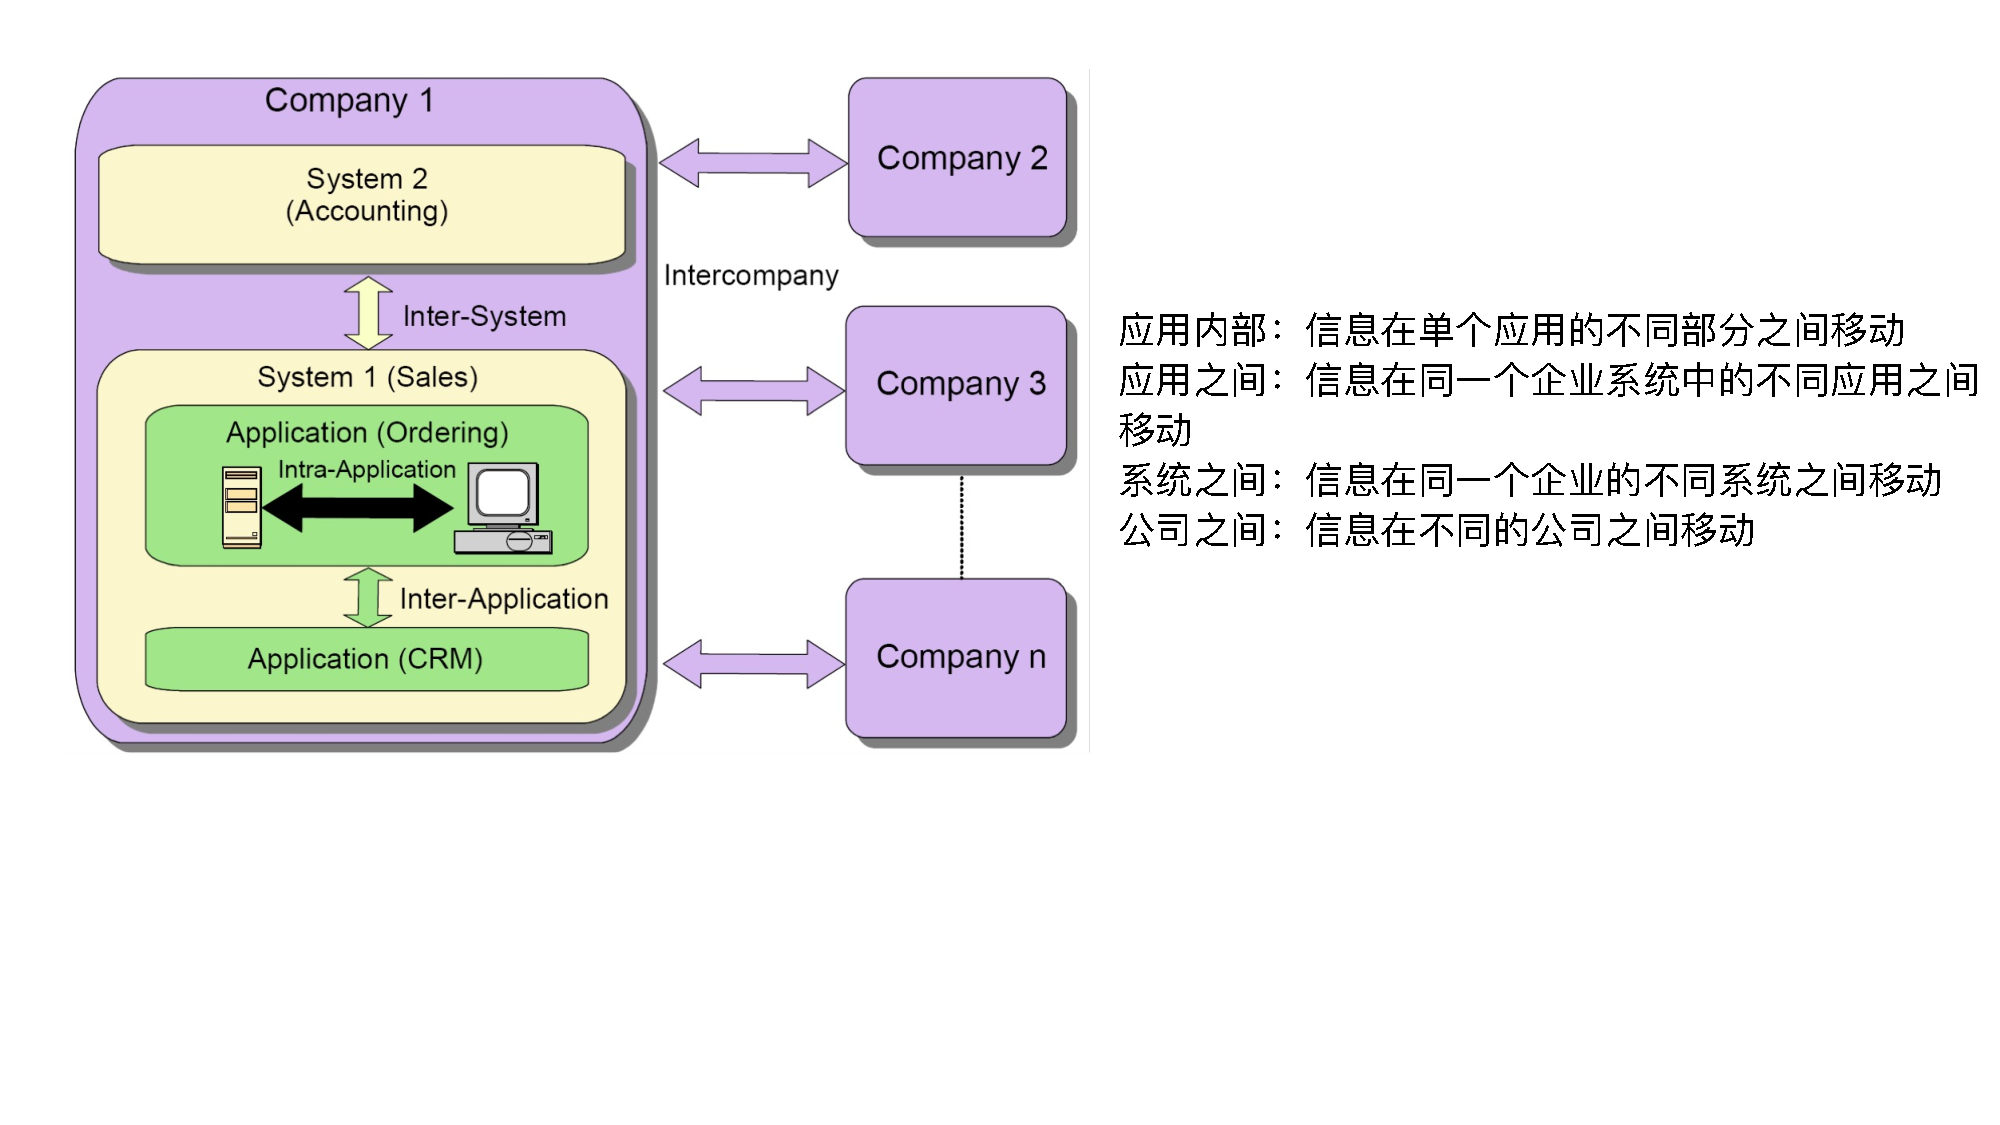
\includegraphics[width=0.95\textwidth]{images/Electronic Information Exchange.pdf}
    \vspace{-1em}
\end{figure}

服务计算中的数据类型
\vspace{-0.8em}
\begin{multicols}{2}
    \begin{itemize}
        \item 使用 XML 消息发布/发现/调用服务
        \item XML 消息交换中的另一个问题是数据类型
        \item 一种方法是用XML 架构脚本验证 XML 消息
        \item 一组XML模式脚本可以在特定的行业中被接受并通过互联网发布,这可以被视为“数据类型标准”
    \end{itemize}
\end{multicols}
\vspace{-1em}

\subsection{XML}
\begin{wraptable}{r}{6.5cm}
    \centering
    \vspace{-1.5em}
    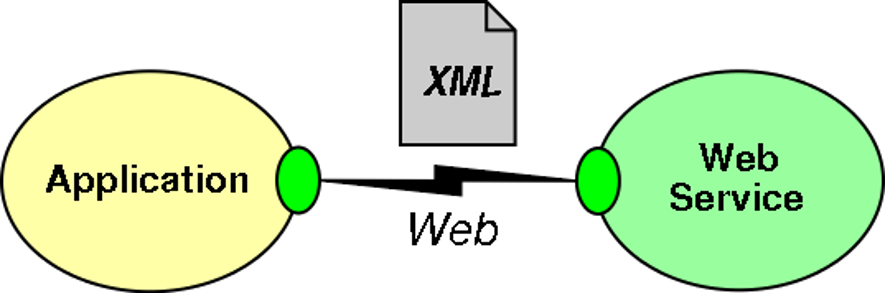
\includegraphics[width=6cm]{images/XML.png}
    \vspace{-1.5em}
\end{wraptable}
XML 是满足一组良好定义规则的格式化文本,主要由标签和文本构成,可以被储存和展现为诸如通过 HTTP 传输的消息、编程语言中的字符串、数据库中的 CLOB(character large object)等文本数据形式。为了方便起见,XML 文档也被用来指应用之间的字节流、数据库中的字段、XML 信息集中的对象集合。

\subsubsection{XML的结构}
XML文档为树状结构
\begin{figure}[H]
    \vspace{-0.5em}
	\centering
	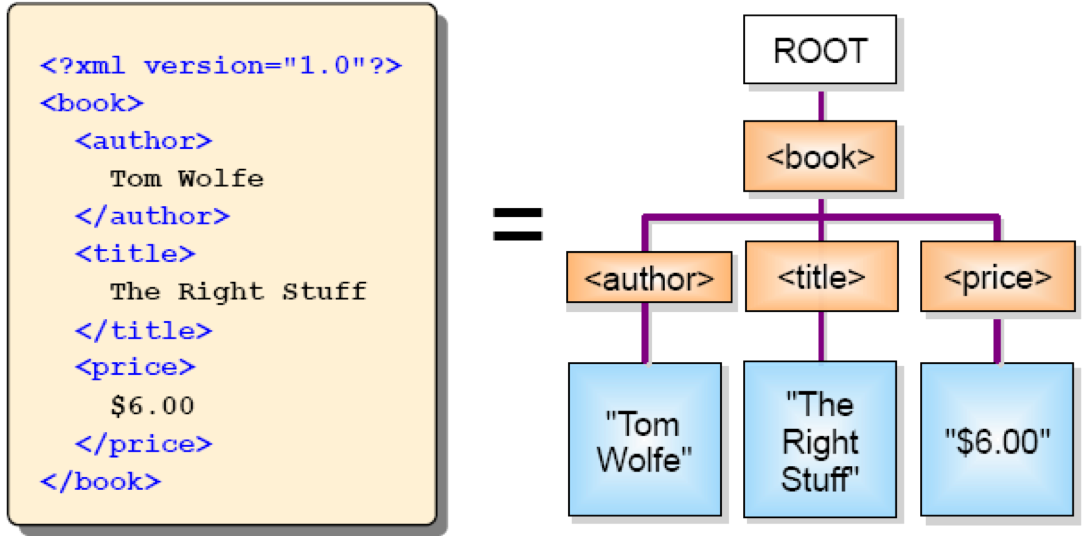
\includegraphics[width=0.7\textwidth]{images/XML文档的树状结构.png}
    \vspace{-1em}
\end{figure}

XML的基本结构:
\begin{figure}[H]
    \vspace{-0.5em}
	\centering
	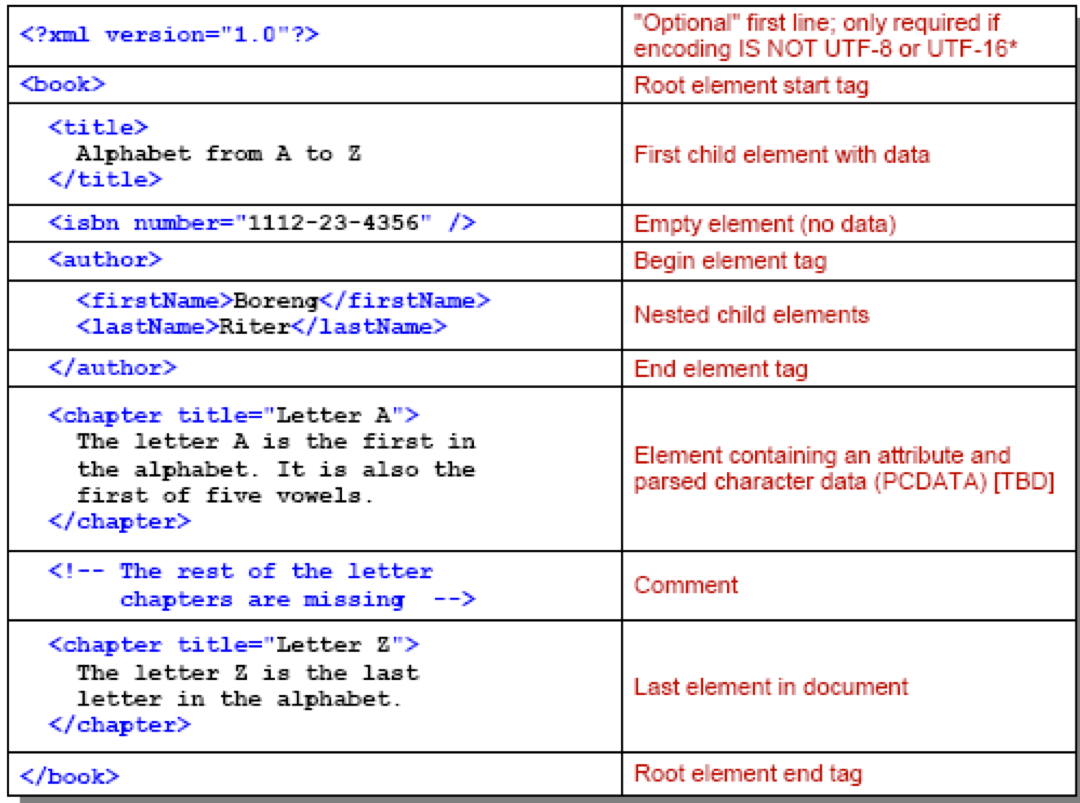
\includegraphics[width=0.7\textwidth]{images/XML的基本结构.png}
    \vspace{-1em}
\end{figure}

\subsubsection{格式良好的XML}
满足$5+1$规则的XML被称为格式良好的XML
\begin{itemize}
    \item 单根元素:所有 XML 文档都只能有一个根元素
    \item 元素标签规则:以开始标签和结束标签来包装元素
    \item 元素嵌套规则:元素标签中间可以嵌套标签
    \item 元素规则
    \begin{itemize}
        \item XML命名:首字母必须是字母或下划线,后街任意长度的字母、数字、连字号等,且不能含有空格,不能以“xml”任何大小写组合作为前缀,XML名称大小写敏感
        \item XML元素内容:XML文档由使用标签对表示的元素、可选属性和可选元素的开始和结束标签之间的数据(可以是文本数据也可以是子元素)所构成。元素内容以两种方式进行处理:
        \begin{itemize}
            \item PCDATA(被解析的字符数据):默认方式,被 XML 解析器进行检查并提取其中的XML内容,这需要对预定义实体进行转义
            \item CDATA(字符数据):采用特殊标记\;\verb|<![CDATA[...]]>|\;进行包装,XML解析器不做处理,只按照字面处理
        \end{itemize}
    \end{itemize}
    \item 元素属性:标签中可以含有属性值键对,用来为元素附加信息,其值必须使用单/双引号括起
    \item XML 声明:可选,出现在 XML 文档中的第一行(\verb|<?xml version="1.0" ?>|,可添加键值对属性)
    \begin{itemize}
        \item encoding属性:用来表达文档所使用的编码,默认为 UTF-8 或 UTF-16
        \item standalone属性:用来表达文档的完整性,即该文档是否依赖于文档外的其他信息,默认为“no”
    \end{itemize}
\end{itemize}


\begin{figure}[H]
	\setcounter{subfigure}{0}
	\centering
	\vspace{-0.5em}	
	\subfloat[单根元素]{
	\begin{minipage}[t]{0.47\linewidth}
	\centering
	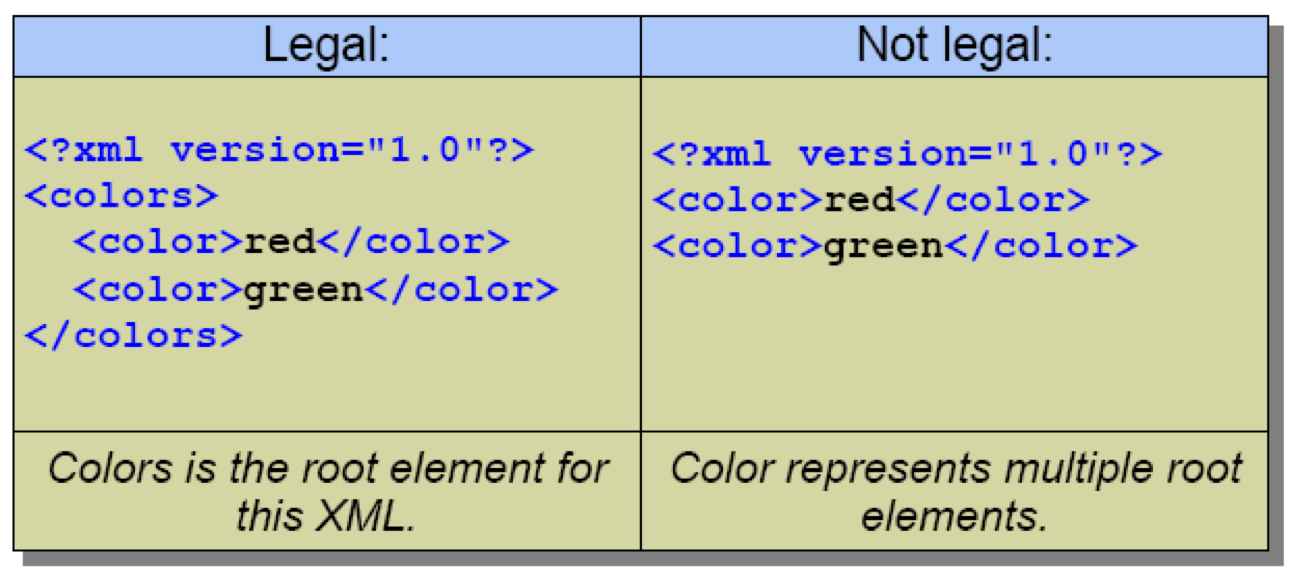
\includegraphics[width=0.97\linewidth]{images/单根元素.png}
	\end{minipage}
	}
    \subfloat[元素嵌套规则]{
	\begin{minipage}[t]{0.47\linewidth}
	\centering
	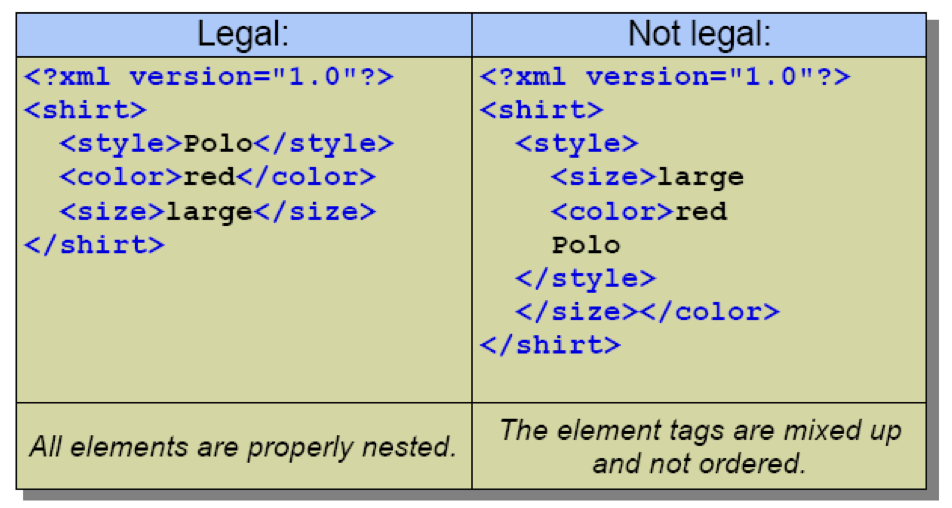
\includegraphics[width=0.93\linewidth]{images/元素嵌套规则.png}
	\end{minipage}
	}
	\centering
	\vspace{-2em}
\end{figure}

\begin{figure}[H]
	\setcounter{subfigure}{2}
	\centering
	\vspace{-0.5em}	
	\subfloat[元素规则:XML命名]{
	\begin{minipage}[t]{0.47\linewidth}
	\centering
	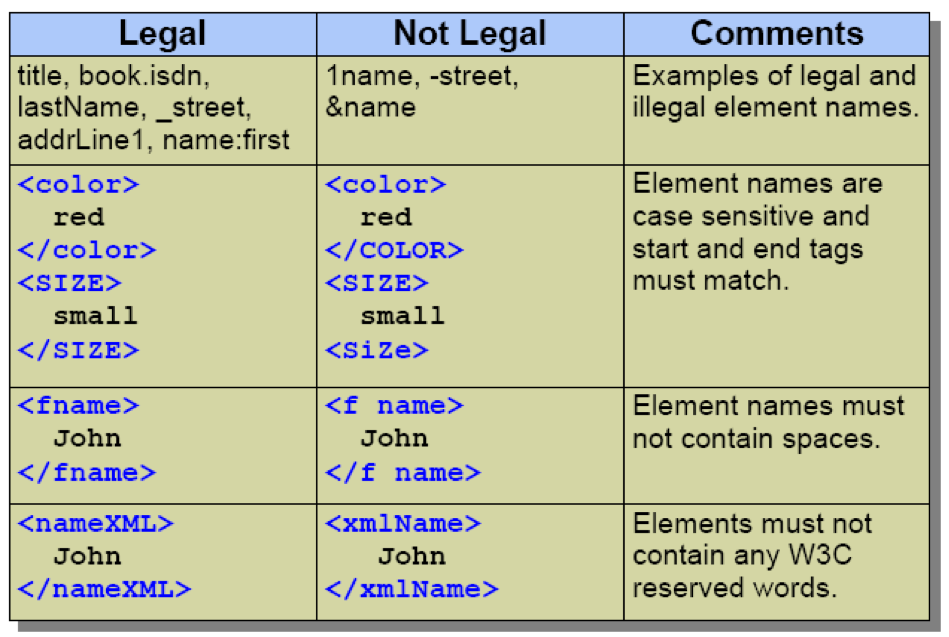
\includegraphics[width=0.97\linewidth]{images/元素规则:XML命名.png}
	\end{minipage}
	}
    \subfloat[元素规则:CDATA]{
	\begin{minipage}[t]{0.47\linewidth}
	\centering
	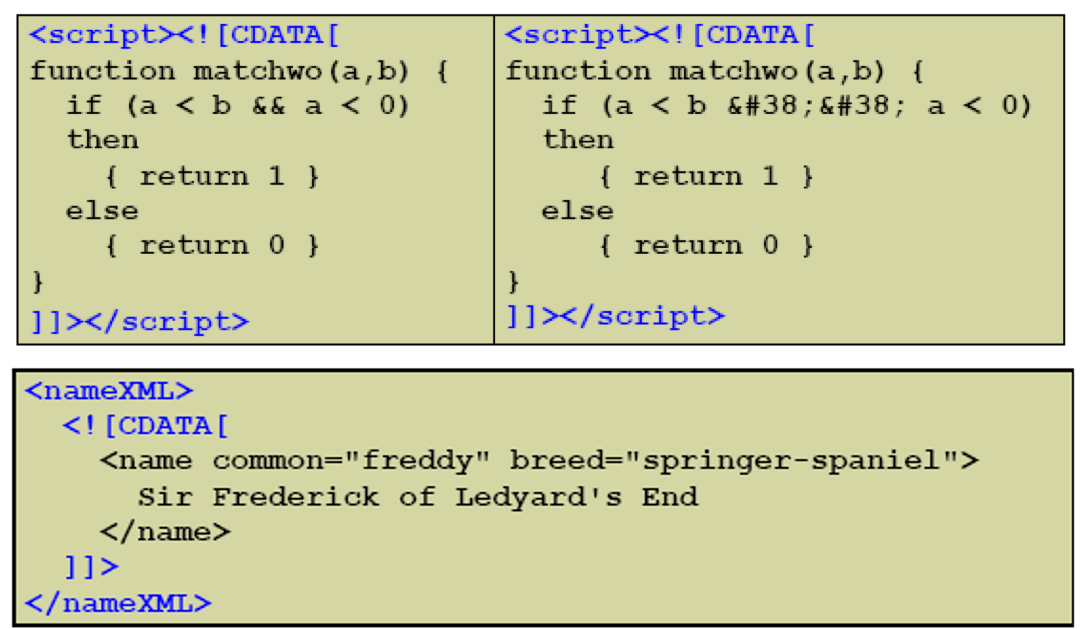
\includegraphics[width=0.97\linewidth]{images/元素规则:CDATA.png}
	\end{minipage}
	}

    \subfloat[元素规则:PCDATA]{
	\begin{minipage}[t]{0.47\linewidth}
	\centering
	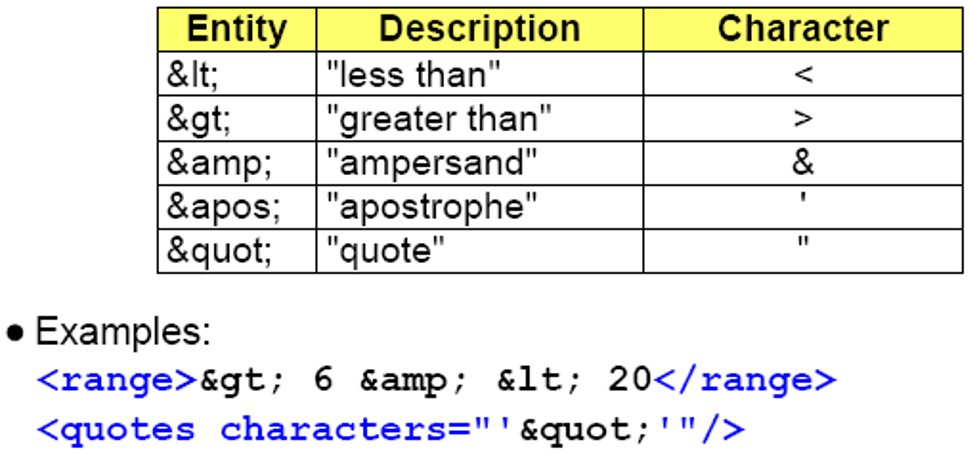
\includegraphics[width=0.97\linewidth]{images/元素规则:PCDATA.png}
	\end{minipage}
	}
    \subfloat[元素属性与XML声明]{
	\begin{minipage}[t]{0.47\linewidth}
	\centering
	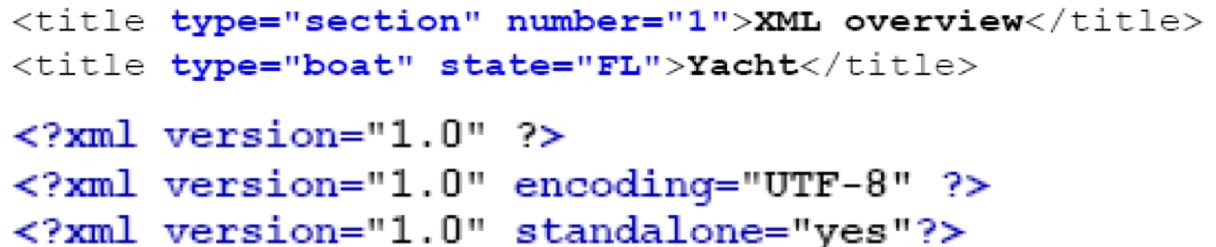
\includegraphics[width=0.97\linewidth]{images/元素属性与XML声明.png}
	\end{minipage}
	}

    \subfloat[注释]{
	\begin{minipage}[t]{0.5\linewidth}
	\centering
	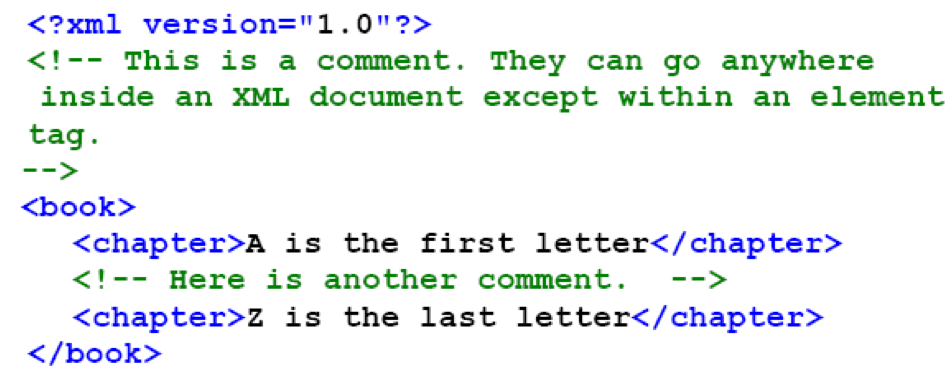
\includegraphics[width=0.97\linewidth]{images/注释.png}
	\end{minipage}
	}
	\centering
	\vspace{-1em}
\end{figure}

一个格式良好的XML文档:
\vspace{-0.8em}
\begin{multicols}{2}
    \begin{itemize}
        \item 由嵌套在另一个XML元素内的XML元素所组成
        \item 具有唯一的根元素
        \item 遵循XML的命名约定
        \item 遵循XML属性引用的规则
        \item 标签被正确终止
    \end{itemize}
\end{multicols}
\vspace{-1em}

所有XML解析器都会检查格式是否良好

有效的XML文档具有一个关联词汇,并遵守该词汇指定的结构规则
\begin{itemize}
    \item 关联词汇通常由DTD或XML Scheme定义
    \item XML解析器可以是验证或非验证的,具体取决于它们是否可以应用关联的语法
    \footnote{XML解析器可以分为两类:验证和非验证。其中,验证解析器可以应用DTD或XML Scheme等关联的语法来验证XML文档是否符合规范。而非验证解析器则不会检查XML文档是否符合规范。换句话说,验证解析器会检查XML文档的语法和结构是否正确,而非验证解析器则只会检查XML文档的格式是否良好。}
\end{itemize}

\subsection{NameSpaces}

\subsubsection{NameSpaces的引入}
NameSpaces的引入:避免在XML文档中出现名称冲突。在XML中,元素和属性都有名称,如果两个不同的元素或属性具有相同的名称,则会导致歧义和混淆。这种冲突的情况在不同的应用程序之间、在不同版本的同一应用程序之间、以及在使用不同的XML词汇表的情况下都可能发生。
\begin{figure}[H]
    \vspace{-0.5em}
	\centering
	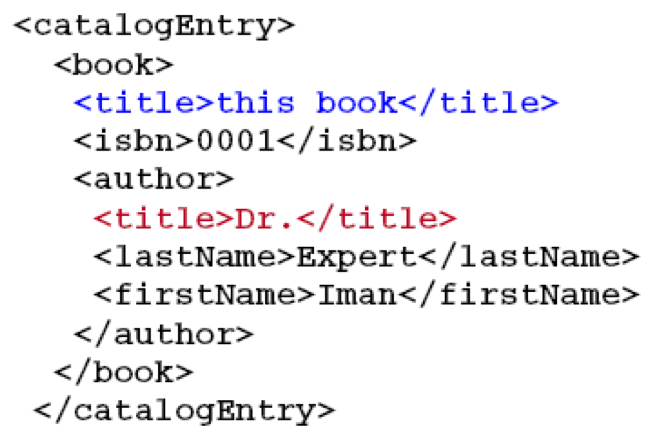
\includegraphics[width=0.38\textwidth]{images/NameSpace的引入.png}
    \vspace{-1em}
\end{figure}

一些可能的解决方案:
\vspace{-0.5em}
\begin{spacing}{1.2}
    \centering
    \begin{longtable}{|m{6cm}<{\centering}|m{8cm}|}
		\hline
		解决方法 & \multicolumn{1}{c|}{说明}  \\ \hline
		采用行业标准的文档格式和命名约定 & 没有哪个行业是孤立的,各行业是相互作用的。这种方法适用于文档级别,一个很好的例子是ebXML,但是元素/属性级别的命名标准过于脆弱 \\ \hline
		使用冗长的元素名称 & 命名变得基本困难,无法知道名称是否已经被使用,而且数据和(或)其模型可能不属于消费应用程序 \\ \hline
		使用一些已经确定为唯一的名称限定符,即域名限定的URI & 域名已经作为唯一标识进行管理和维护。这种方法很有前途,并被发展成为XML命名空间 \\ \hline
    \end{longtable}
	\end{spacing}
\vspace{-1em}

从概念上讲,每个元素名称和属性名称都可以表示为:URI $+$名称,例如\sverb|<title>|\;可能会变成
\begin{lstlisting}
<http://www.library.com/books:title>
\end{lstlisting}
这种格式存在两个问题:
\vspace{-0.8em}
\begin{multicols}{2}
    \begin{itemize}
        \item 它在1.0规范下不是良好格式的XML
        \item 需要输入很多字符
    \end{itemize}
\end{multicols}
\vspace{-1em}

如果能够为URI创建一个同义词,并用该同义词替换URI的出现次数,则输入的字符数量将减少,并且如果处理正确,则结果将与XML 1.0兼容
\begin{itemize}
	\item 例如标记\sverb|books="http://www.library.com/books"|\;然后直接使用 \sverb|<books:title>|
	\item 这个概念形成了XML命名空间规范的基础
\end{itemize}


\subsubsection{QNames}
引入名称空间后,元素名称和属性名称转换为两部分名称,即QNames(Qualified Names)。QNames 用来在 XML 中担任元素名称和属性名称。
\begin{figure}[H]
    \vspace{-0.5em}
	\centering
	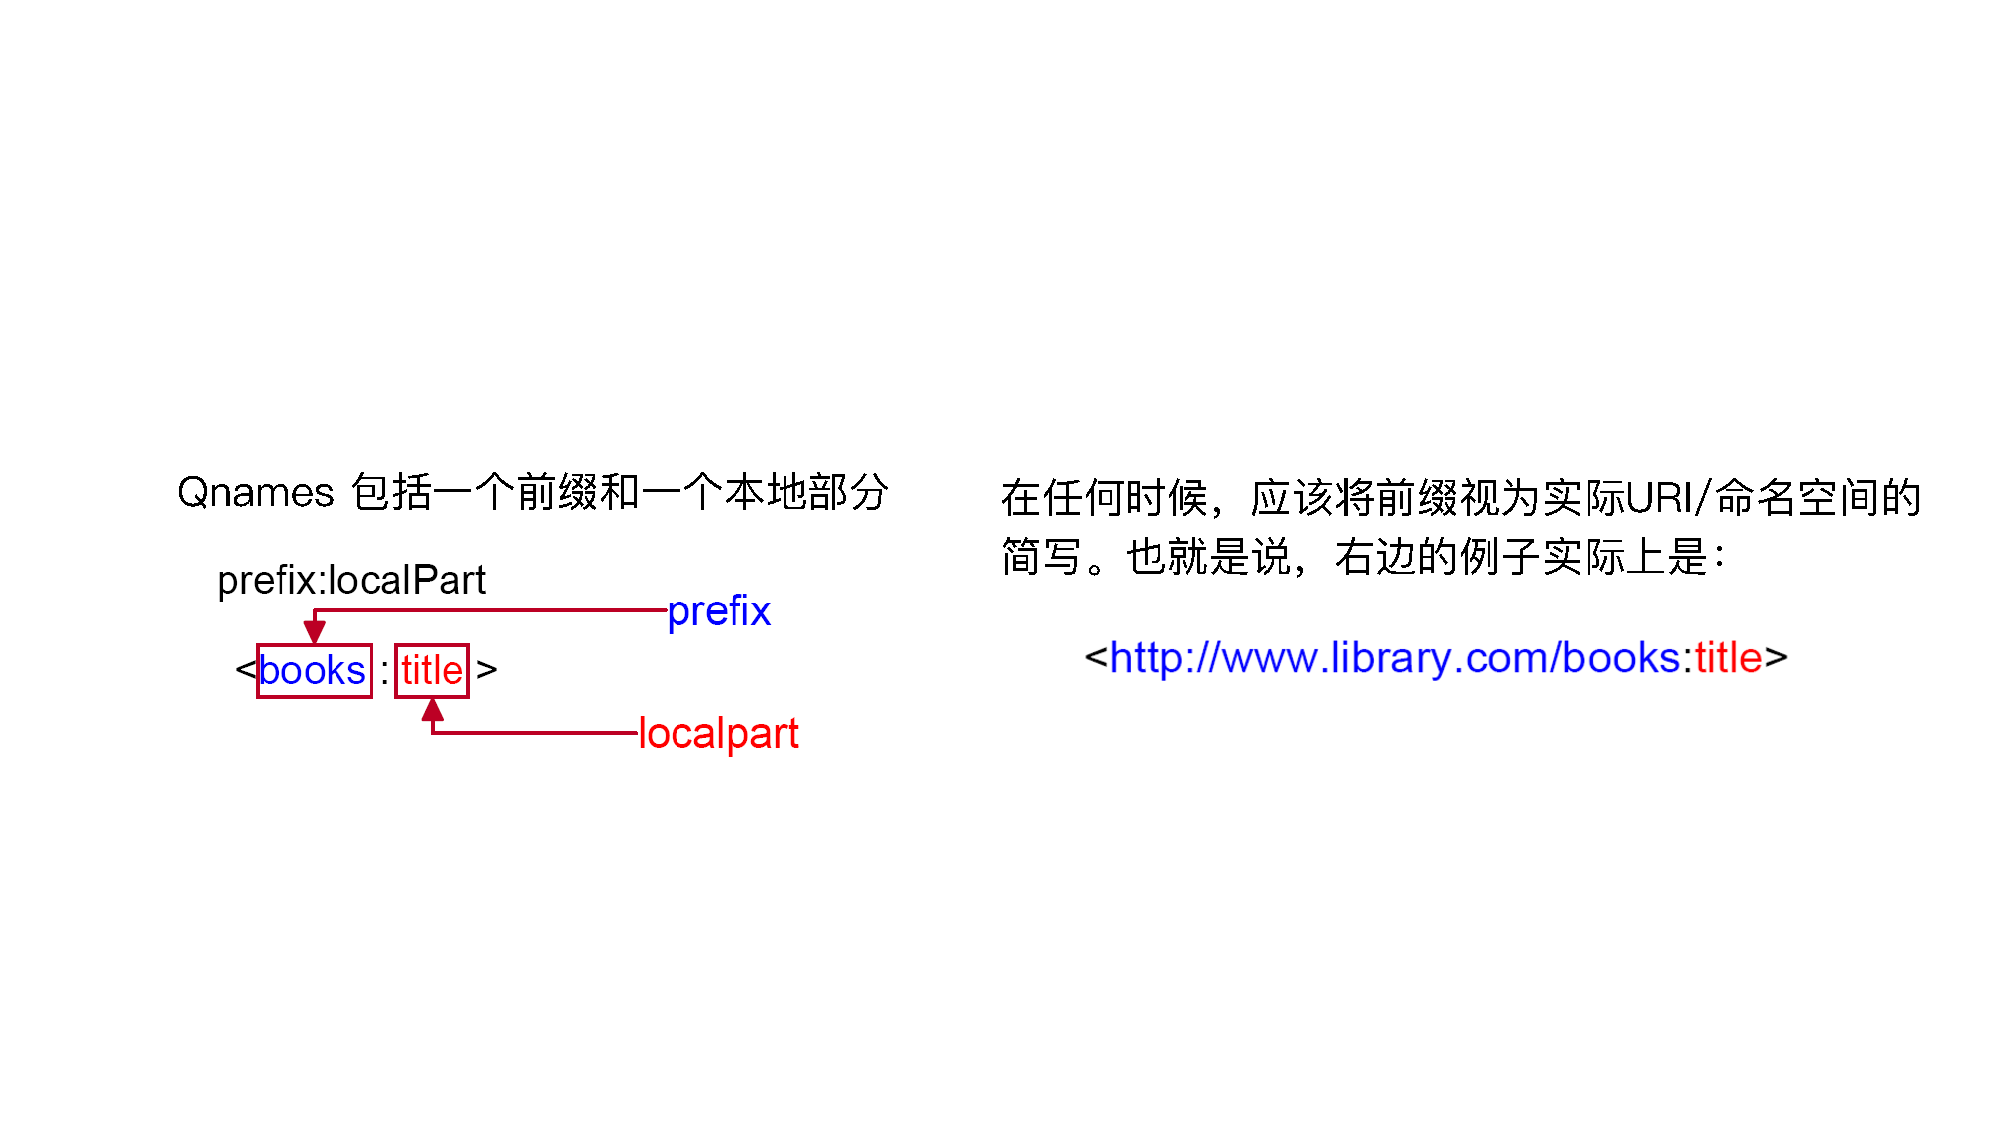
\includegraphics[width=0.95\textwidth]{images/Qnames.pdf}
    \vspace{-1em}
\end{figure}

\subsubsection{Namespaces的声明}
声明Namespaces的语法为
\begin{lstlisting}
<prefix:elementName xmlns:prefix='URI'>
\end{lstlisting}

下面的例子声明了命名空间\;\url{http://www.library.com/books},并将其分配一个前缀为“books”,并将book元素标识为该命名空间的成员
\begin{lstlisting}
<books:book
	xmlns:books='http://www.library.com/books'/>
\end{lstlisting}
属性也可以属于命名空间。与元素一样,属性也要按以下方式加前缀
\begin{lstlisting}
<books:book
	xmlns:books='http://www.library.com/books'
	books:hardcover='true'/>
\end{lstlisting}

\subsubsection{名称空间作用域}
\begin{itemize}
	\item 名称空间前缀的作用域为定义该名称空间的元素(含嵌套的子元素和所隶属的属性)
	\item 名称空间前缀可以在嵌套的子元素中进行重新定义
\end{itemize}

\begin{lstlisting}
<books:book
	xmlns:book='http://www.library.com/books'
	books:hardcover='true'>
		<books:title>
			Tom Sawyer
		</books:title>
</books:book>
\end{lstlisting}

\subsubsection{默认名称空间}
在大多数元素隶属于相同的名称空间时,可以使用默认名称空间
\begin{lstlisting}
<elementName xmlns='URI'/>
\end{lstlisting}
\begin{itemize}
	\item 在默认名称空间的作用域内,可以使用QName来定义隶属于其他名称空间的元素
	\item 默认名称空间不作用于属性,如不使用QName,默认情况下,属性没有名称空间
	\begin{itemize}
		\item 属性隶属于某一个特定的元素,在元素为一确定的情况下,隶属于该元素的拥有不同名称的属性也是唯一确定的
	\end{itemize}
\end{itemize}

\begin{lstlisting}
<book xmlns='http://www.library.com/books'
	xmlns:books='http://www.library.com/books'
	books:hardcover='true'>
  <title>Tom Sawyer</title>
</book>
<!-- book 和 title 隶属于同一个名称空间 -->
\end{lstlisting}

\subsubsection{拥有多个名称空间的XML文档}
\begin{figure}[H]
    \vspace{-0.5em}
	\centering
	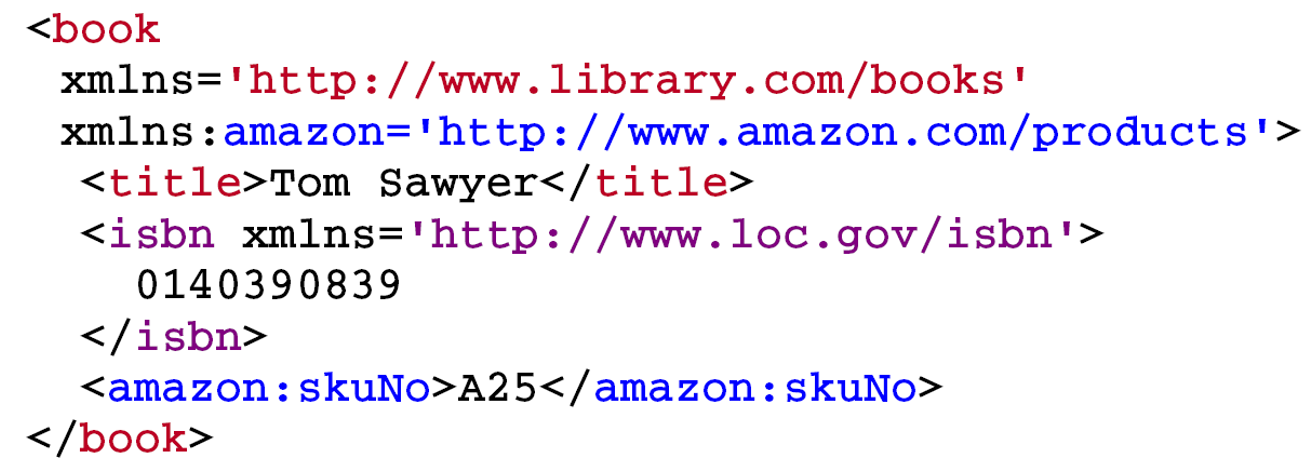
\includegraphics[width=0.7\textwidth]{images/拥有多个名称空间的XML文档}
    \vspace{-1em}
\end{figure}

\subsubsection{没有名称空间的元素}
使用\sverb|xmlns=""|\;用以重置默认名称空间,定义没有名称空间的元素。
\begin{figure}[H]
    \vspace{-0.5em}
	\centering
	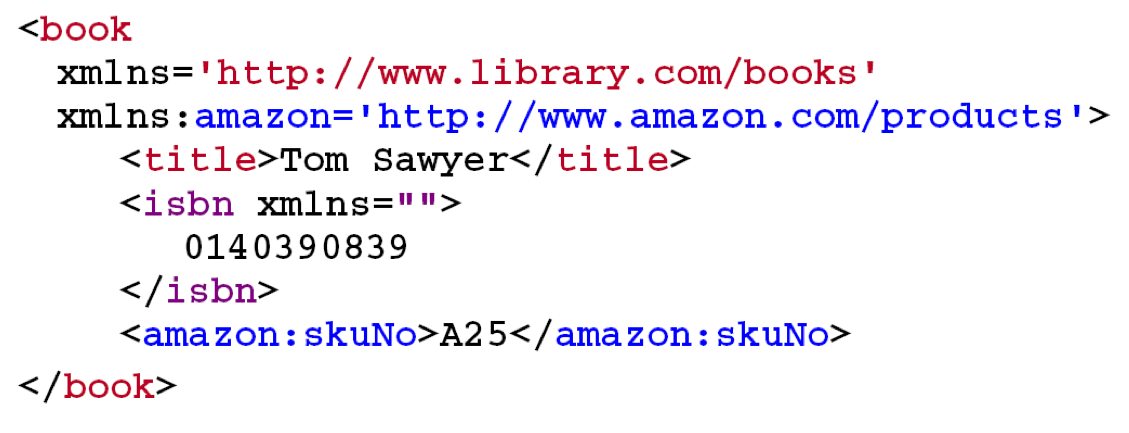
\includegraphics[width=0.65\textwidth]{images/没有名称空间的元素}
    \vspace{-1em}
\end{figure}

\subsubsection{属性与名称空间}
\vspace{-0.8em}
\begin{multicols}{2}
    \begin{itemize}
        \item 属性不受默认命名空间的影响
        \item 特定元素中的属性应各不相同
    \end{itemize}
\end{multicols}
\vspace{-1em}
\begin{figure}[H]
    \vspace{-0.5em}
	\centering
	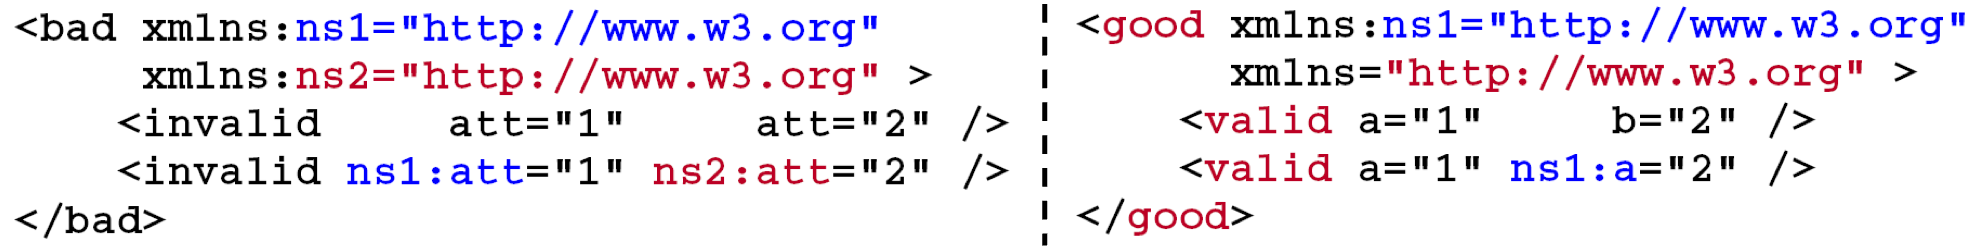
\includegraphics[width=0.96\textwidth]{images/属性与名称空间}
    \vspace{-1em}
\end{figure}

\subsection{XML Schema}

\subsubsection{为什么要引入XML Schema}
从业务角度来看
\vspace{-0.8em}
\begin{multicols}{2}
    \begin{itemize}
        \item 需要增加数据的表示能力
		\item 需要融合来源于不同组织的词汇表
		\item 通过提升通信效率的方式以减少集成的成本
    \end{itemize}
\end{multicols}
\vspace{-1em}

从技术角度来看
\vspace{-0.8em}
\begin{multicols}{2}
    \begin{itemize}
		\item 采用具体的定义验证 XML 文档
		\item 采用 XML 语法
		\item 定义数据结构和约束条件
		\item 支持名称空间
		\item 表达数据元素之间的关系
    \end{itemize}
\end{multicols}
\vspace{-1em}


\subsubsection{XML Schema的结构}
\begin{figure}[H]
    \vspace{-0.5em}
	\centering
	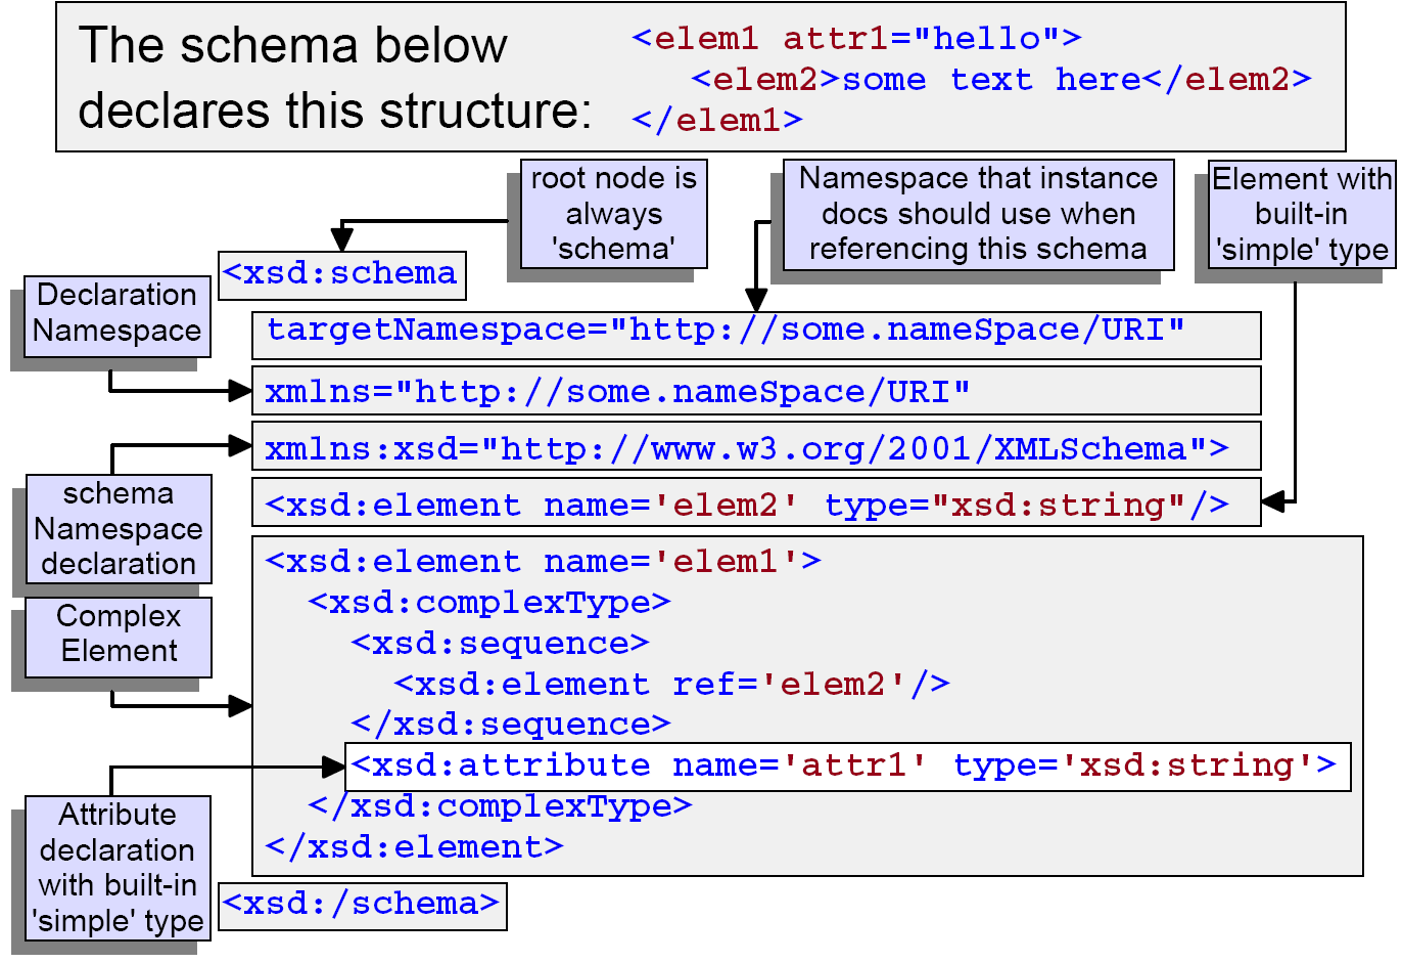
\includegraphics[width=0.7\textwidth]{images/XML Schema的结构.png}
    \vspace{-2em}
\end{figure}


\subsubsection{XML Schema的特点}
\vspace{-0.8em}
\begin{multicols}{2}
	\begin{itemize}
		\item 使用XML实例语法来定义XML文档的结构
		\item 在表达元素和属性内容的数据类型语义方面更加出色
		\item 支持命名空间
		\item 将数据类型的定义与元素和属性的声明分开
		\item 支持表示数据的唯一性和关系
	\end{itemize}
\end{multicols}
\vspace{-1em}


\subsubsection{元素声明}
\paragraph*{定义简单元素}~{} \par
采用已有的类型定义(内建或已定义)来说明元素
\begin{lstlisting}
<xsd:element name='quantity'
			type='xsd:noNegativeInteger'
			minOccurs='1' maxOccurs='1'/>
\end{lstlisting}

其中,name指定元素名称,type指定元素值的类型,minOccurs、maxOccurs指定元素至少、至多出现的次数。类型必须带有命名空间限定符。如果类型未与模式的默认命名空间关联,则必须使用表示正确命名空间的命名空间前缀进行限定。

\textbf{例:}minOccurs与maxOccurs
\begin{figure}[H]
    \vspace{-0.5em}
	\centering
	\includegraphics[width=\textwidth]{images/minOccurs与maxOccurs.png}
    \vspace{-3em}
\end{figure}

\paragraph*{声明子元素}~{} \par
采用排序符定义元素中的子元素
\begin{figure}[H]
    \vspace{-0.5em}
	\centering
	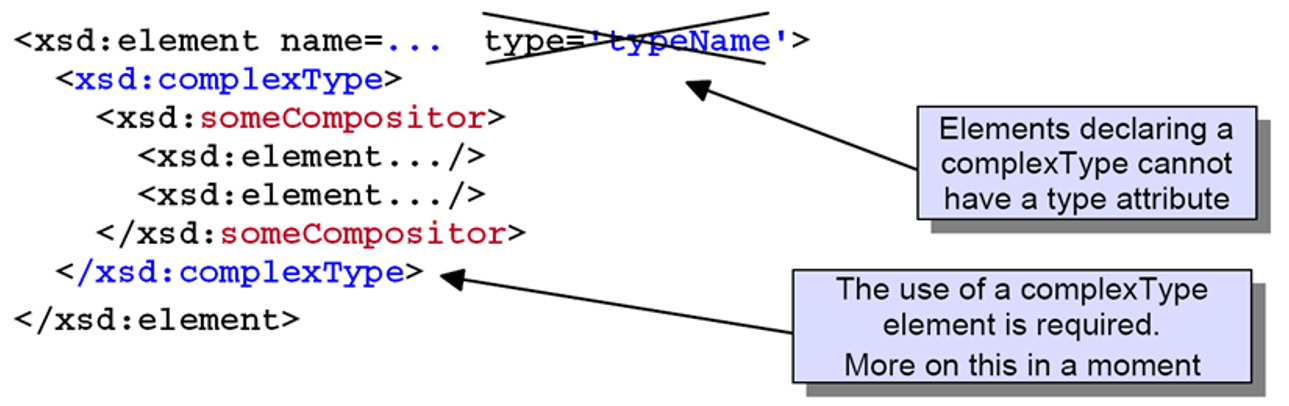
\includegraphics[width=0.75\textwidth]{images/采用排序符定义元素中的子元素}
    \vspace{-1em}
\end{figure}

\textbf{例:}按序列出现的firstName和lastName
\begin{lstlisting}
<xsd:sequence>
 	<xsd:element name='firstName' type='xsd:string'/>
	<xsd:element name='lastName' type='xsd:string'/>
</xsd:sequence>
\end{lstlisting}

\textbf{例:}maidenName和cityOfBirth选择其一
\begin{lstlisting}
<xsd:choice>
	<xsd:element name='maidenName' type='xsd:string'/>
	<xsd:element name='cityOfBirth' type='xsd:string'/>
</xsd:choice>
\end{lstlisting}

\textbf{例:}height和weight以任意顺序出现
\begin{lstlisting}
<xsd:all>
	<xsd:element name='height' type='xsd:float'/>
	<xsd:element name='weight' type='xsd:float'/>
</xsd:all>
\end{lstlisting}

\paragraph*{声明属性}~{} \par
\begin{lstlisting}
<xsd:element name=''>
	<xsd:complexType>
		<xsd:attribute name='attName' type='aSimpleType' fixed|defalut='value' use='...'/>
	</xsd:complexType>
</xsd:element>
\end{lstlisting}
在\sverb|xsd:attribute|\;声明中使用的一些有用(可选)属性包括:
\begin{itemize}
	\item Use:值可以是required(必需的),prohibited(禁止的)和optional(可选的),默认值为optional
	\item Default:当属性不存在时,提供属性的默认值
	\item Fixed:将属性值固定为指定的值
\end{itemize}

对于属性的一些规则:
\vspace{-0.8em}
\begin{multicols}{2}
	\begin{itemize}
		\item 属性类型必须是simpleType(即非元素类型)
		\item \verb|xsd:attribute|\;不能同时存在fixed和default
		\item 当提供默认值时,Use属性必须为“optional”或不存在
	\end{itemize}
\end{multicols}
\vspace{-1em}

\textbf{例:}声明属性
\begin{figure}[H]
    \vspace{-0.5em}
	\centering
	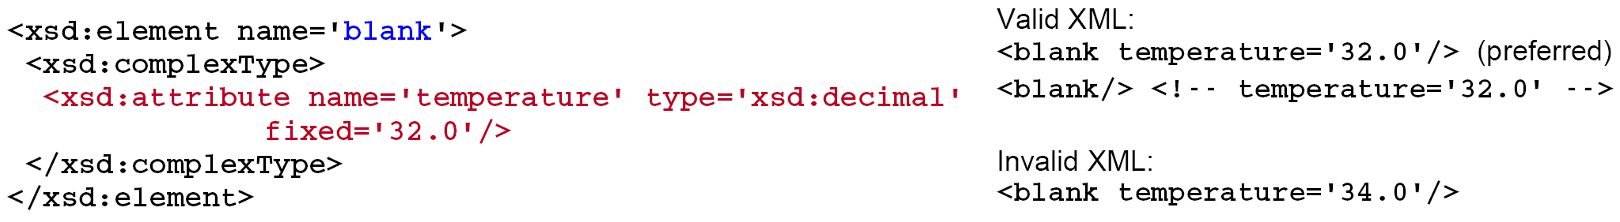
\includegraphics[width=0.98\textwidth]{images/声明属性}
    \vspace{-1em}
\end{figure}

\textbf{例:}同时含有子元素和属性的元素声明
\begin{figure}[H]
    \vspace{-0.5em}
	\centering
	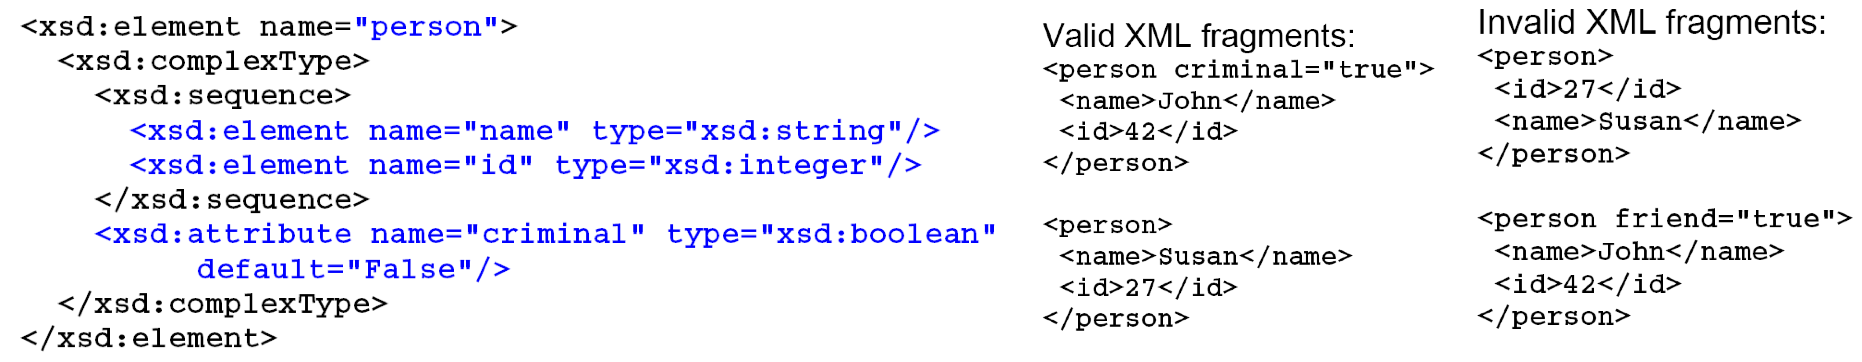
\includegraphics[width=\textwidth]{images/同时含有子元素和属性的元素声明}
    \vspace{-2em}
\end{figure}

\paragraph*{属性组}~{} \par
如果一组属性经常一起使用,则可以创建一个属性组来形式化关系,并避免需要在多个位置声明相同的属性。
\begin{figure}[H]
    \vspace{-0.5em}
	\centering
	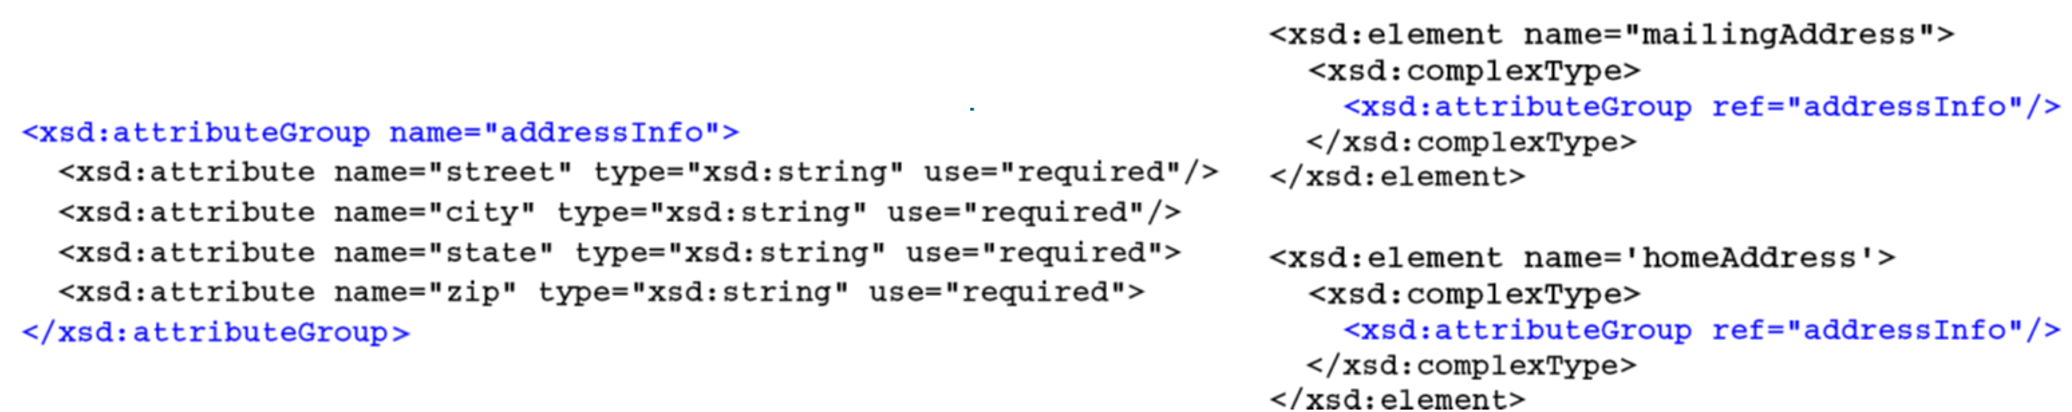
\includegraphics[width=\textwidth]{images/属性组}
    \vspace{-2em}
\end{figure}

\subsubsection{XML Schema类型系统}
XML Schema 类型系统分为两个不同的类型类别:简单类型和复杂类型
\vspace{-0.8em}
\begin{multicols}{2}
    \begin{itemize}
		\item 简单类型
		\begin{itemize}
			\item 不能有属性或子元素
			\item 是 XML Schema 类型语言的基本元素
			\item 用于定义其他类型,包括复杂和简单类型
			\item 包括 40 多个预定义的简单类型
		\end{itemize}
		\item 复杂类型
		\begin{itemize}
			\item 可以有属性
			\item 可以用于定义其他复杂类型
			\item 不能用于定义简单类型
			\item 可以有子元素
		\end{itemize}
    \end{itemize}
\end{multicols}
\vspace{-1em}

\paragraph*{取值约束}~{} \par
\begin{figure}[H]
    \vspace{-0.5em}
	\centering
	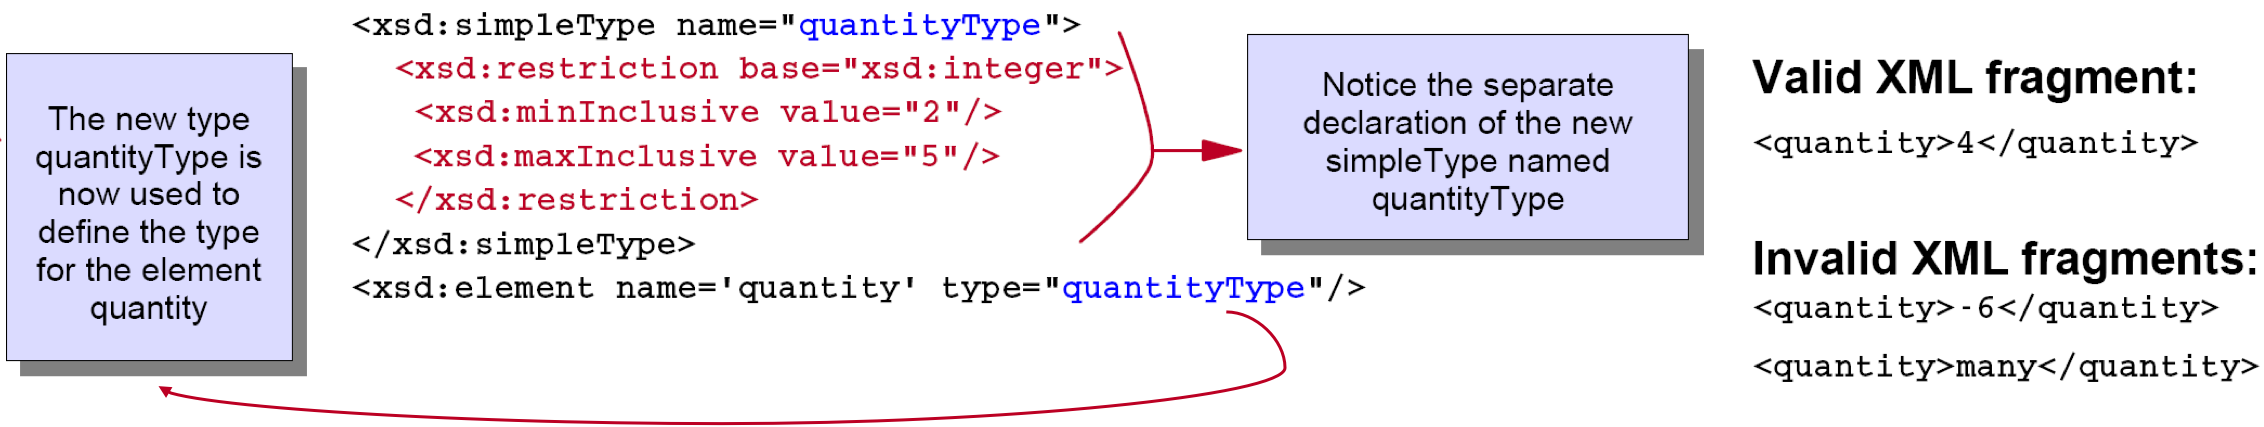
\includegraphics[width=\textwidth]{images/取值约束}
    \vspace{-2em}
\end{figure}

\paragraph*{枚举约束}~{} \par
\begin{figure}[H]
    \vspace{-0.5em}
	\centering
	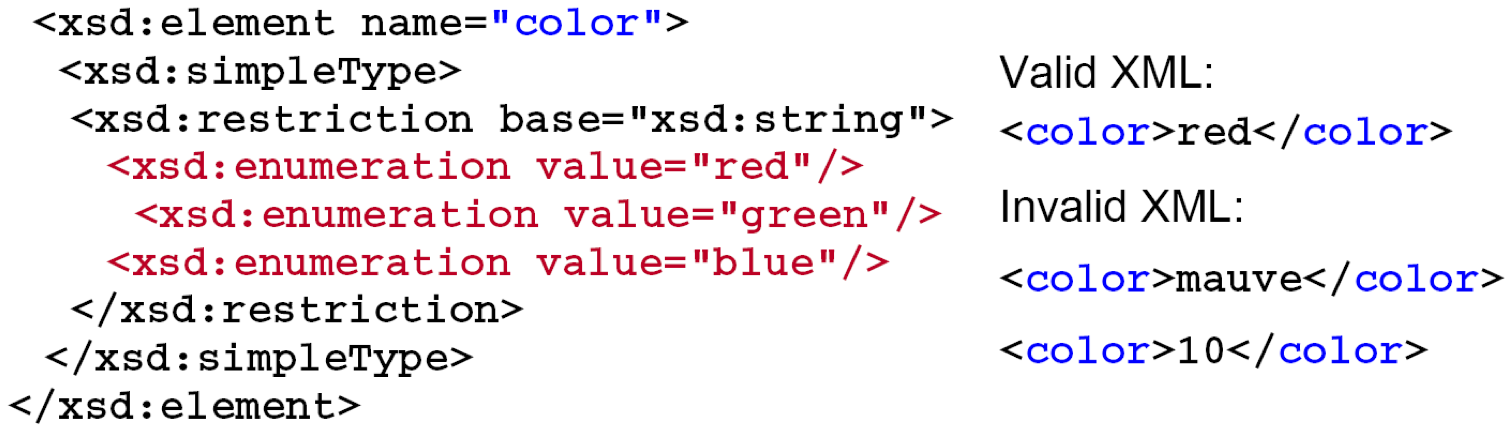
\includegraphics[width=0.65\textwidth]{images/枚举约束}
    \vspace{-1em}
\end{figure}

\paragraph*{simpleContent}~{} \par
simpleContent元素必须包含一个restriction或extension元素,这些元素用于定义该元素的简单类型。restriction用于限制元素的取值范围,而extension则用于扩展已有的简单类型。

\begin{lstlisting}
<xsd:complexType name="simpleContentType">
	<xsd:simpleContent>
		<xsd:extension base="xsd:...">
		...
		</xsd:extension>
	</xsd:simpleContent>
</xsd:complexType>
\end{lstlisting}

\begin{figure}[H]
    \vspace{-0.5em}
	\centering
	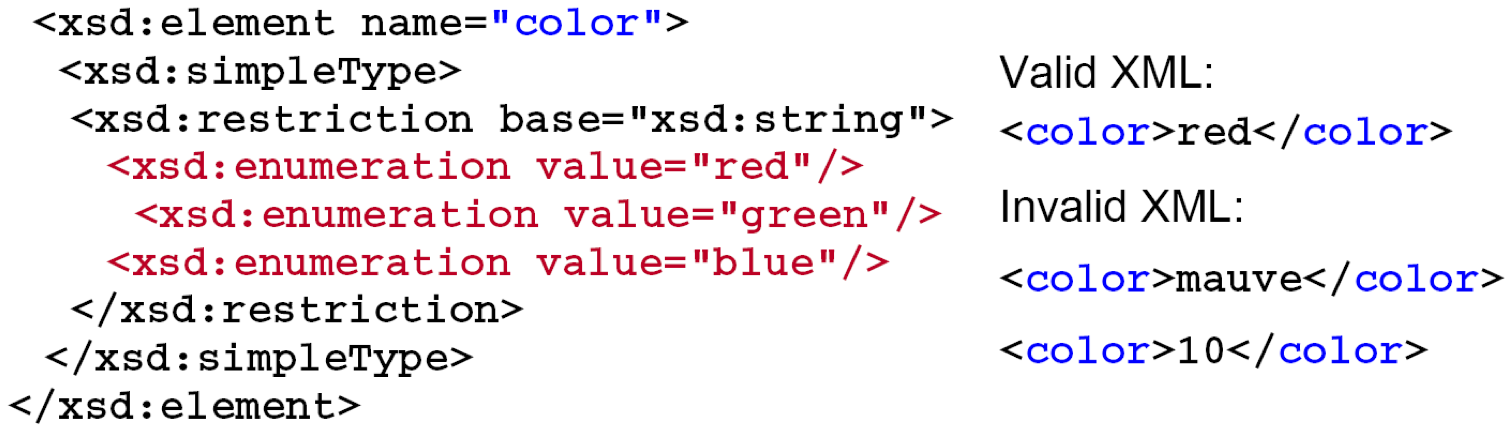
\includegraphics[width=0.75\textwidth]{images/枚举约束}
    \vspace{-1em}
\end{figure}

\paragraph*{element only}~{} \par
当一个类型被声明为element only,就指定该类型的实例只能包含元素,而不能包含文本或字符数据。也就是说,该类型的实例不允许出现文本节点或CDATA节点,只能是元素节点。
\begin{lstlisting}
<xsd:complexType name="elementOnlyType">
	<xsd:sequence>
		<xsd:element name="firstName" type="xsd:string"/>
		<xsd:element name="lastName" type="xsd:string"/>
	</xsd:sequence>
<xsd:complexType>
\end{lstlisting}

\paragraph*{Mixed}~{} \par
当一个类型被声明为mixed,它指定该类型的实例可以包含元素、文本或字符数据,或它们的任意组合。也就是说,该类型的实例允许同时包含元素节点和文本节点或CDATA节点。
\begin{lstlisting}
<xsd:complexType name=mixedType" mnixed=true">
	<xsd:sequence>
		<xsd:element name="firstName" type="xsd:string"/>
		<xsd:element name="lastName" type="xsd:string"/>
</xsd:sequence>
</xsd:complexType>
\end{lstlisting}

\paragraph*{具名类型与匿名类型}~{} \par
\begin{itemize}
	\item 在XML Schema中,一个元素可以有一个具名类型或一个匿名类型。具名类型是通过名称来引用的,而匿名类型是定义元素时内联定义的类型。
	\item 具名类型是为多个元素定义的,可以被引用并重复使用,而匿名类型仅用于单个元素。具名类型可以在文档中的多个地方重复使用,而匿名类型只能在定义它们的元素上使用。
	\item 具名类型可以提高XML Schema的可重用性和可维护性,而匿名类型则可以减少模式定义时的冗余。
\end{itemize}

\begin{figure}[H]
	\setcounter{subfigure}{0}
	\centering
	\vspace{-1.5em}	
	\subfloat[具名类型]{
	\begin{minipage}[t]{0.41\linewidth}
	\centering
	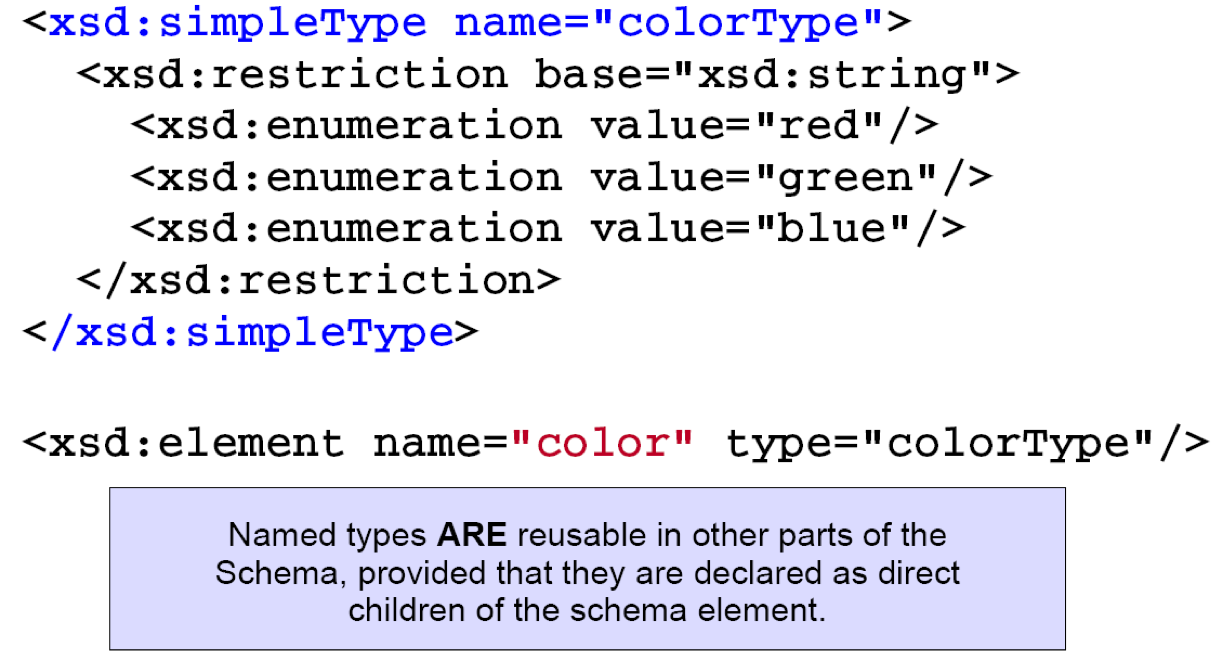
\includegraphics[width=0.97\linewidth]{images/具名类型.png}
	\end{minipage}
	}
    \subfloat[匿名类型]{
	\begin{minipage}[t]{0.53\linewidth}
	\centering
	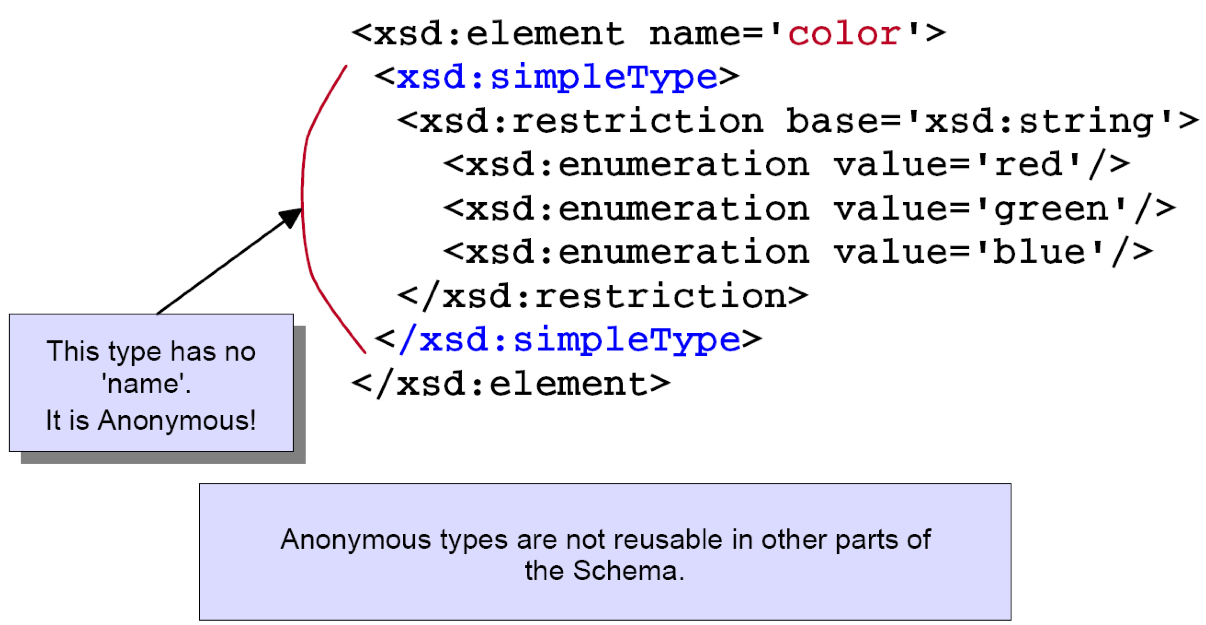
\includegraphics[width=0.97\linewidth]{images/匿名类型.png}
	\end{minipage}
	}
	\centering
	\vspace{-1em}
\end{figure}

匿名类型也可以用在属性声明中
\begin{figure}[H]
    \vspace{-0.5em}
	\centering
	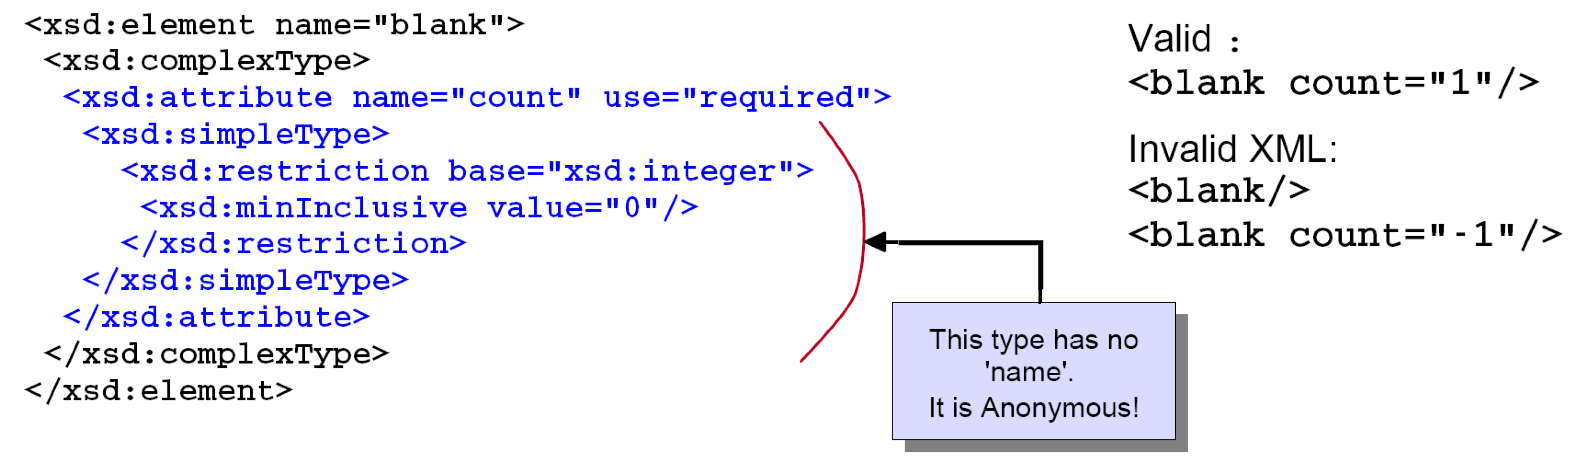
\includegraphics[width=0.85\textwidth]{images/属性声明中的匿名类型.png}
    \vspace{-2.5em}
\end{figure}

\paragraph*{全局类型与局部类型}~{} \par
\begin{itemize}
	\item 类型可以在元素中声明为局部类型。匿名类型是局部类型。
	\item 类型可以在模式元素的直接子级中全局声明。命名类型是全局类型。
	\item 只有顶级类型可以命名和重复使用。
\end{itemize}

\begin{figure}[H]
    \vspace{-0.5em}
	\centering
	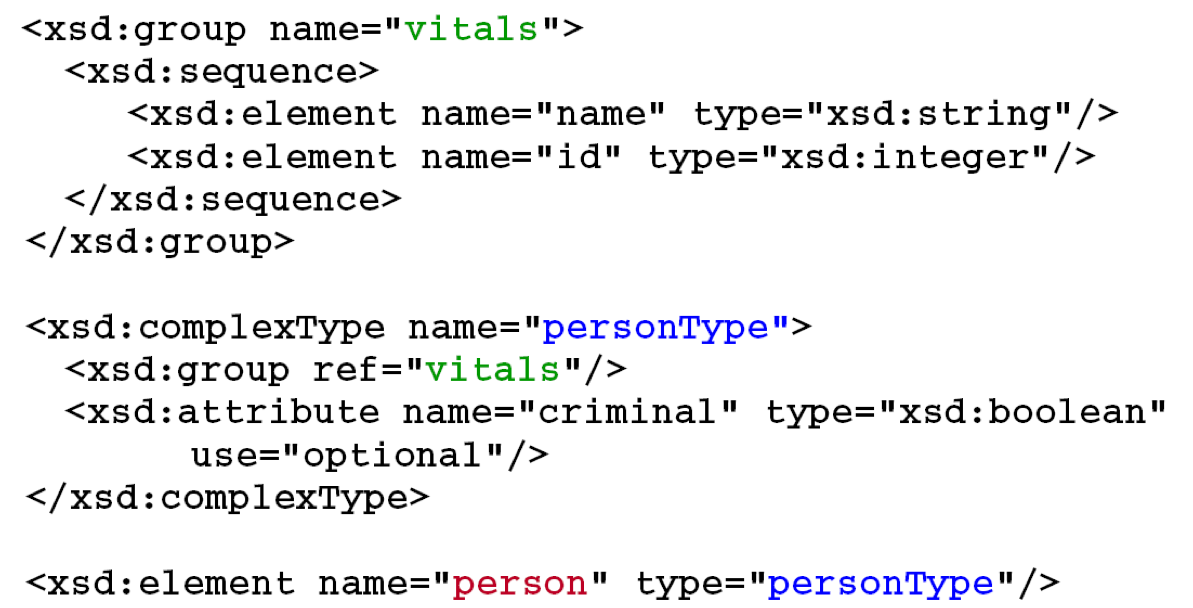
\includegraphics[width=0.65\textwidth]{images/全局声明.png}
    \vspace{-1em}
\end{figure}

\subsubsection{在XML中说明名称空间}
\begin{lstlisting}
<xsd:schema
	xmlns="http://www.ibm.com/schemas/WD03/target"
	xmlns:xsd="http://www.w3.org/2001/XMLSchema"
	targetNamespace="http://www.ibm.com/Schemas/WD03/target" elementFormDefault="qualified">
	<xsd:element name="quantity" type="xsd:integer"/>
</xsd:schema>
\end{lstlisting}
在schema脚本中所定义的元素,理论上来说都应该被放置或关联到一个特定的名称空间
\begin{itemize}
	\item targetNamespace中的URI就是当前这个schema脚本中所定义的元素(在上例中为quantity)隶属的名称空间
\end{itemize}


\subsubsection{寻找XML Schema}
\begin{figure}[H]
	\setcounter{subfigure}{0}
	\centering
	\vspace{-1.5em}	
	\subfloat{
	\begin{minipage}[c]{0.47\linewidth}
	\centering
	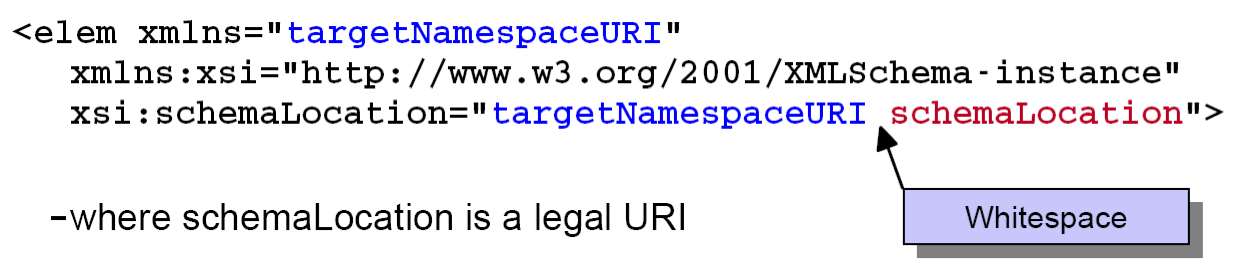
\includegraphics[width=0.97\linewidth]{images/寻找XML Schema.png}
	\end{minipage}
	}
    \subfloat{
	\begin{minipage}[c]{0.47\linewidth}
	\centering
	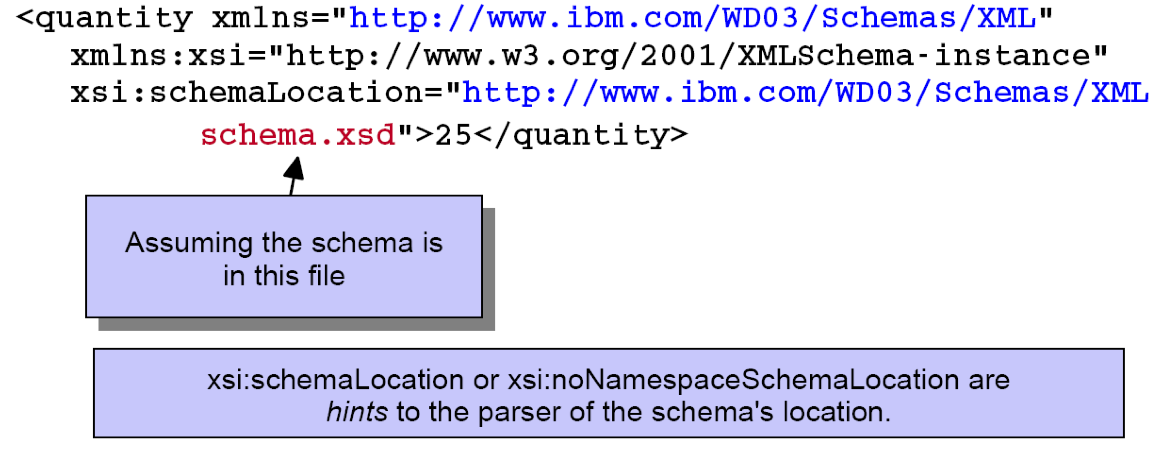
\includegraphics[width=0.97\linewidth]{images/寻找XML Schema2.png}
	\end{minipage}
	}
	\centering
	\vspace{-1em}
\end{figure}

使用XML Schema Instance(xsi)用于指定 XML 实例文档与 XML Schema 之间关联的命名空间前缀。它是由 XML Schema 规范定义的,用于表示 XML 实例文档中使用的元素和属性是基于哪个 XML Schema 定义的。

通过在 XML 实例文档中使用该命名空间前缀和schemaLocation属性,可以指定 XML Schema 文件的位置和名称,从而使 XML 解析器能够在验证 XML 实例文档时使用正确的 XML Schema 文件。

\textbf{例:}下面的 XML 实例文档中使用了xsi命名空间前缀,并使用schemaLocation属性指定了XML Schema文件的位置:
\begin{lstlisting}
<?xml version="1.0" encoding="UTF-8"?>
<root xmlns:xsi="http://www.w3.org/2001/XMLSchema-instance"
      xsi:schemaLocation="http://www.example.com/schema/schema.xsd">
  <element1>value1</element1>
  <element2>value2</element2>
</root>
\end{lstlisting}
